\documentclass[10pt, a4paper, twocolumn]{jsarticle}
%
\usepackage{amsmath,amssymb}
\usepackage{bm}
\usepackage{graphicx}
\usepackage{ascmac}
\usepackage{subfigure}
\usepackage{multicol}
\usepackage{setspace}
\usepackage{mediabb}
\usepackage{float}
\usepackage{latexsym}
\usepackage{url}
\usepackage{cite}
\usepackage[top=30truemm,bottom=30truemm,left=16truemm,right=16truemm]{geometry}
%
\setlength{\textwidth}{178truemm}
\setlength{\textheight}{39\baselineskip}
\addtolength{\textheight}{\topskip}
\setlength{\voffset}{-0.5in}
\setlength{\headsep}{0.3in}
%
\renewcommand{\baselinestretch}{1.0}
\renewcommand{\figurename}{Fig.}
\renewcommand{\tablename}{Table.}
\renewcommand{\headfont}{\bfseries}


\begin{document}
\twocolumn[
\begin{screen}
\begin{flushleft}
融合情報学輪講資料\hspace{\fill}2014/07/25
\end{flushleft}
\begin{center}
{\Large  Multipath TCP適用時のデータセンターネットワークでのショートフローに対する改善  \\
Improving the effect of the short flows in the data center network with
Multipath TCP}
\end{center}
\begin{flushleft}
工学系研究科 電気系工学専攻 関谷研究室\hspace{\fill}修士課程2年 37-136482 藤居 翔吾
\end{flushleft}
\end{screen}
\vspace{0.5cm}
]
\begin{spacing}{0.7}
\begin{bfseries}
\begin{itshape}
Abstract-
\end{itshape}

As increasing the number of servers in a datacenter, the effective network
topology for utilization of massive computer clusters has been studied.
Recently, using MPTCP for the beneficial use has been tackled this problem.
As another solution, distributed processing system enabled to handle big data.
Today's the technique of distributed processing is that massive workers
process data followed by the query from the master nodes.
As the result, a large quantity of short flow is generated in a datacenter
network.
MPTCP can achieve the effective consumptions of the resources with multipath,
but a researcher reported MPTCP causes the delay of flow completion for short
flows.
In this paper, I verified the MPTCP's effects for short flows in the datacenter
network with the traffic of distributed processing service.
There are two negative factors, bottleneck at aggregation switch and multiplexed
flow patterns in one host, and I clarified short flow delays arise under what
circumstances.


\vspace{0.5cm}
\begin{itshape}
Index-
\end{itshape}
Multipath TCP, Short flow, Flow completion time, FatTree topology, Datacenter
network\end{bfseries}
\end{spacing}
\vspace{0.5cm}
\section{Introduction}
\label{sec:intro}

多様な端末がネットワークに接続できるようになり, 様々な端末から大量かつ多種多様なデータの取得が可能となった.
特にトラフィックデータ量の増加傾向は顕著で, 18$\sim$24ヶ月単位で総データ容量が2倍になるという予測がされている~\cite{IBM_rep}.
またFacebookでは, 300ペタバイト以上のデータ量を保有しており, 1日あたりに1ペタバイトのデータを解析している~\cite{presto}.
このように近年では, クラウドによるビッグデータの活用が着目され, ウェブ検索エンジンやSNS(Social Networking Service)など,
リアルタイムに近いレスポンスを返すような場面において使われ始めている.
そのようなクラウドサービスには近年, より良いユーザーエクスペリエンスの要求が高まってきており,
Amazonでは100[ms]の遅延により売り上げが1\%下がる, といった報告~\cite{amazon}があるように, レスポンス遅延の影響は深刻な問題となっている.
そのため, 大規模データをより高速に解析することが求められており, データセンターではサーバの運用台数が増加の一途をたどっている.
しかし, 大量の計算機資源から最大限の性能を引き出すためには,
従来の仕組みではデータセンター内トラフィックに対してトラフィックが集中する問題に対応できないため,
計算機資源を有効活用するための研究が盛んに行われている\cite{mapreduce, dryad, fattree, bcube, vl2,
dctcp, improving, detail, p_fab}.
そのようなスケーラビリティ拡大には, ネットワークトポロジー, アプリケーション, プロトコルに対するアプローチがある.

ネットワークトポロジーを改良するアプローチでは, 従来の単純な階層構造では,
データセンター内で発生するトラフィックに対して帯域が最大限割り当てられない~\cite{fattree}.
そのため, 近年ではそのようなトラフィックに対してスイッチを多段に構成することで帯域を有効利用するトポロジーが提案されている.

大量のデータの処理速度を改良するアプローチでは,
分散処理のためにpartition-aggregate計算モデルが提案されている.
MapReduce~\cite{mapreduce}, Dryad~\cite{dryad}等の分散処理フレームワークは,
この計算モデルに従っており, 今日の大規模クラウドサービスにおいては, 必要不可欠である.

プロトコルを改良するアプローチでは,
従来のTCPを拡張したMultipath TCP
(MPTCP)~\cite{mptcp}をデータセンターネットワークに用いる提案がされている~\cite{fattree,bcube,vl2}.
MPTCPを用いることにより, 複数の経路を同時に利用し, スループットを向上させることが期待されている.

しかし, 分散処理フレームワークを用いることで, フローサイズの小さい大量のQueryが発生し, MPTCPは,
フローサイズの小さいトラフィック(ショートフロー)に対しては, TCPよりも性能が劣化する問題が報告された~\cite{improving}.

このような背景から, 大規模データセンターネットワークへのMPTCP適用時のショートフロー遅延の問題は並列分散処理アプリケーションの性能の面で深刻な問題である.
そこで本論文では, データセンターネットワークにおけるショートフローに対するMPTCPの影響を検証し,
その原因を分析する.
特に, ns-3シミュレーションを用いたトラフィック解析結果を示し, どのような状況でショートフローが遅延するのかその要因を示す.

% 本稿では, \ref{sec:related}章でMPTCPによるデータセンターネットワークモデルに関する先行研究を示し,
% \ref{sec:mptcp}章ではMPTCPの詳細を述べる.
% \ref{sec:fattree}章では近年提案されたネットワークトポロジーを紹介し, \ref{sec:traffic_scenario}章では
% データセンター内のトラフィックに関する特性を示す.
% そして, \ref{sec:reproduction}章では報告された問題を検証し,
% \ref{sec:evaluation}章ではデータセンターネットワークでのMPTCPの性能について評価, 考察する.
% 最後に, \ref{sec:conclude}章で本稿での検証結果についてまとめる.

\section{関連研究}
\label{sec:related}
本章では, これまでに報告されている複数経路利用によるフロー完結時間短縮化技術について簡潔に述べ, その優位性や問題点を示す.

2010年にAlizadehらによって, データセンターネットワーク特有のトラフィックパターンに特化して,
パラメータを決定するアルゴリズムが提案された~\cite{dctcp}.
データセンター特有のバースト性のあるトラフィックが引き起こす問題点として, キューの生成によるキューイング遅延, キュー溢れによるパケットロス,
スイッチのバッファに掛かる負荷がある.
これらの問題に対し, キューの蓄積を制御するためのバッファサイズをアルゴリズムから動的に設定することで,
大部分のキューの伝送時間を短縮することを可能にした.
これらの問題に対し, 経由するスイッチにおいて, ECN(Explicit Congestion Notification)によってエンドホストに輻輳を通知し,
キューの大部分が占有される前にウィンドウサイズを動的に変化させ, キューサイズを小さく保つアルゴリズムによって,
大部分のキューの伝送時間を短縮することを可能にした.
しかし, 大規模計算資源を想定したトポロジーにおける検証がされておらず, また各ネットワークデバイスに細かなチューニングを必要とするため,
大規模データセンターでは運用面での問題がある.
さらに, サイズの大きいフローの割合の大きいトラフィックの中では, その影響によりウィンドウサイズを小さくする制御が働くため,
サイズの小さいフローの完結時間への効果が小さい, と報告されている~\cite{p_fab}.

2011年にCostinらによって, MPTCPを用いたデータセンターネットワークモデルが提案された~\cite{improving}.
近年の大規模計算資源を有効活用するために提案されたネットワークトポロジーでは,
高性能なデバイスや特殊な機器を必要とせず, 汎用デバイスのみを用いてホスト同士の通信の際に経路が複数用意されている.
これまでは通信に使わない経路をセカンダリ経路として利用することで, 耐障害性を持たせていたのに対し, 提案されたデータセンターモデルでは,
MPTCPを用い複数経路を同時に利用する事で, 耐障害性を保ちながら, 帯域を最大限利用する事を可能にした.
また, 様々なトポロジーにMPTCPを適用することで, 従来のTCPよりも高いスループットが出せることを示した.
しかし, サイズの小さいフロー($\leq70KB$)のフロー完結時間に着目すると, TCPよりも時間がかかるという問題点があった.

2012年にZarsらによって, 複数レイヤー間でトラフィックを監視し,
しきい値を設定することによるフロー完結時間の短縮化技術を提案した~\cite{detail}.
サイズの異なるフローが混在するネットワークにおいては, サイズが小さいフローがサイズの大きいフローに圧迫され,
伝送遅延が大きくなる問題があったが, この提案では, データリンク層からアプリケーション層までの各層が, 相互にトラフィックを監視する機能をスイッチに実装し,
優先度をつけ, バッファサイズを調整することで, フロー完結時間の悪化を抑えることを可能にした.
しかし, 実験ではClick~\cite{click}を用いて実装を行っており, 現実世界での全てのネットワーク機器の置き換えが必要となるので, 実現は難しい.

以上で述べたことをまとめると, 近年のデータセンターネットワークに対して, 以下のような要求が考えられる.
\begin{itemize}
  \item 大規模計算機を有効活用するトポロジーの利用
  \item 分散処理の際に発生する大量のサイズの小さいフローの送信時間の短縮
  \item 特殊な実装やデバイスを用いず, シームレスな運用の実現
\end{itemize}

\section{データセンターネットワーク}
\label{sec:datacenter}
本章では, データセンターネットワークを構成する技術に関して, その概要を述べる.
\subsection{Multipath TCP}
MPTCPは, 一つの経路でデータ転送するTCPを拡張し, 複数のインタフェース,
あるいは複数のポートを用いてデータ転送をするプロトコルである~\cite{mptcp}.
クライアントが複数のIPアドレスを持っていた場合, 新たにサブフロー\footnote{複数のTCPコネクションの内,
ある一つのコネクションにおけるフロー}のコネクションが確立される.
追加されたサブフローは, クライアントの持つインターフェースが1つの場合, 同じIPアドレスで異なる送受信ポートを用いる.
インターフェースを複数持つ場合には, 異なるIPアドレスの組み合わせで通信を行う.
ルーティングに関しては, 複数の宛先IPアドレス, 送信元アドレスからそれぞれ経路決定される.
このように, アプリケーション層より下のレイヤーのみで複数の経路を使ってデータ転送を行うため,
アプリケーション側がMPTCPでの通信を意識することなくデータ転送ができる.

MPTCPでは, サブフローが, それぞれのシーケンス領域を持ち, 経路状態に合わせて輻輳制御をするCoupled Congestion Control
Algorithmがある~\cite{cong}.
このアルゴリズムには, TCPと同様にAIMD(additive-increase and
multiplicative-decrease)による輻輳制御がサブフロー単位で行われる.
以下にAIMDアルゴリズムを示す.

\begin{itemize}
\item サブフロー $r$において,
1ACKごとにウィンドウサイズ$\omega_{r}$をmin$(\frac{\alpha}{\omega_{total}},
\frac{1}{\omega_r})$増加させる.
\item サブフロー $r$において, パケットロス時にウィンドウサイズ$\omega_r$を$\frac{\omega_r}{2}$へ減少させる.
\end{itemize}
ここで, $\omega_{total}$は全てのサブフローのウィンドウサイズの総和, $\alpha$は送信速度の増加量を示すパラメータで,
以下のように定義される~\cite{cong}.

\vspace{-2mm}
\begin{eqnarray}
 \alpha = \omega_{total} \times
\frac{\displaystyle \max_{r} \frac{w_r}{RTT^2_r}}{\displaystyle
(\sum_{r}\frac{w_r}{RTT_r})^2}
\label{alpha}
\vspace{-2mm}
\end{eqnarray}

ここで, $RTT_r$はサブフロー$r$でのラウンドトリップ時間を示している.
MPTCPでの輻輳制御には二つの性質ある.
一つは, サブフローのウィンドウサイズは, 全てのウィンドウサイズの大きさに依存するということである.
これにより, 混雑したサブリンクにおいては, ウィンドウサイズが抑えられ, ロードバランスができる.
二つ目は, MPTCPのアルゴリズムによって, TCPでの輻輳制御よりも悪化する事を回避している事である.
しかし, もし複数のサブフローがそれぞれ混雑のないサブリンクを利用する場合, いずれかのコネクションが帯域を占有する可能性がある.

\subsection{FatTreeトポロジーとMPTCPによるデータセンターモデル}
\label{sec:fattree}
この節では, データセンターを構成する要素について述べる.
\subsubsection{トポロジー}
\label{subsec:topology}
従来のデータセンターモデルでは, HostがEdgeスイッチにつながり,
これらのスイッチがAggregationスイッチに集約され,
coreスイッチに接続するといったように, 階層的にトポロジーを形成していた~\cite{fattree}.
このような単純な階層構造を持つトポロジーは, トラフィックの大部分がデータセンター外の通信には有効であった.
しかし, 今日のようなデータセンター内で生じるトラフィックが大半を占める場合, 帯域の割当が適切でなくなる.
このような, データセンター内のトラフィックが主であれば, 階層型のトポロジーはボトルネックを引き起こす可能性がある.
近年の研究~\cite{fattree,bcube,vl2}では, トラフィックがデータセンター内に集中した時の問題を, 物理的なアプローチとして,
トポロジーを工夫する事で解消を試みている.

図\ref{fig:fattree}のように, FatTree~\cite{fattree}では, Coreスイッチを複数用いる事で,
物理パスの最大帯域を供給する.
また, 比較的狭い帯域の経路と汎用的な性能のスイッチを多数用いる.

このようなトポロジーを用いる事で, データセンター内のトラフィックに対し, 帯域を十分に使う事ができる.
しかしこのような密な配置により, 複数の経路が形成され, ルーティングをどのように決定すべきかという問題も生じる事となる~\cite{improving}.
例えば図\ref{fig:fattree}のようなFatTreeトポロジーでは, 4通りの経路が考えられる.
これら複数の経路をリンクエラー時の冗長性を持たせる目的だけでなく, 性能向上に活用することが求められている.
\begin{figure}[h]
    \begin{center}
    \includegraphics[autoebb, width=210pt]{./img/fattree_topology.pdf}
    \caption{Fattree topology}
    \label{fig:fattree}
    \end{center}
\end{figure}
% \begin{figure}[h]
%     \begin{center}
%     \includegraphics[autoebb, width=180pt]{./img/hierarchy_topology.pdf}
%     \caption{階層型ネットワークトポロジー}
%     \caption{Hierarchical network topology}
%     \label{fig:hierarchical}
%     \end{center}
% \end{figure}

% \begin{figure}[h]
% \begin{minipage}{0.5\hsize}
% \begin{center}
% \includegraphics[autoebb, width=110pt]{./img/fattree_topology.pdf}
% \end{center}
% \caption{FatTreeトポロジー}
% \caption{Fattree topology}
% \label{fig:fattree}
% \end{minipage}
% \begin{minipage}{0.5\hsize}
% \begin{center}
% \includegraphics[autoebb, width=110pt]{./img/bcube.pdf}
% \end{center}
% \caption{BCubeトポロジー}
% \caption{BCube topology}
% \label{fig:bcube}
% \end{minipage}
% \end{figure}

\subsection{データセンターにおけるトラフィックシナリオ}
\label{sec:traffic_scenario}
大量の計算機資源を有効活用するためには,
並列分散処理フレームワークを用いられ, 一般的に図\ref{fig:part_aggr}に示すようにpartition-aggregate構造をとる.
並列分散処理フレームワークでは, 多数の処理ノードと分散処理の制御をする管理ノードから構成されており, 管理ノードからQueryが発行され,
分散処理がそれを受け取り,レスポンスを返す.
このとき, トラフィックパターンが  (1){\it Query traffic}, (2){\it Short message
traffic}, (3){\it Backgroung traffic}の3つに分類される~\cite{dctcp}.

{\bf Query traffic. }Query trafficとは, 大規模計算処理を分割して並列処理する際に,
aggregatorノードから処理ノードへ具体的な処理を割り当てるためのトラフィックである.
Query trafficの特徴は, 非常に小さいフローサイズ(2KB$\sim$20KB)で、処理全体の遅延に非常に強く影響を及ぼす事である.
また並列分散処理システムの構成上, Query trafficはms$\sim \mu$s単位でQueryが生成され,
バースト性を持つと言える~\cite{dctcp}.

{\bf Short message traffic. } Short message trafficとは,
処理ノードの動作を制御するためのトラフィックである.
Short message trafficの特徴は, フローサイズは50KB$\sim$1MBで, Query
trafficと同様に処理全体の遅延に影響を及ぼすという事である.
しかし, Querry trafficほどのフロー数は生成されず, 生成時間間隔も秒単位である.

{\bf Backgroung traffic. }Backgroung trafficは,
各処理ノードへ更新データを送信するトラフィックである.
Backgroung trafficの特徴は,フローサイズが1MB$\sim$50MBと大きいことにある.
さらに, その生成時間間隔は大きい.
また, Backgroung trafficでの更新データは, 処理精度の向上に寄与するが, 処理に必須ではないので,
処理全体の遅延にはつながらない.
また, Alizadehらは, 実際のデータセンターのトラフィックでは, Background trafficが発生する数は少ないが,
全体の通信量の大部分がBackgroung trafficによって占められていると報告しており,
経路全体へ影響を及ぼす可能性があることを示している~\cite{traffic}.

つまり, データセンターネットワークのトラフィックのうち, 分散処理開始時に生成されるQuery trafficが遅延すると,
処理全体に対し遅延を引き起こすので, Query trafficのフロー完結時間は極めて重要なメトリックである.

\begin{figure}[h]
    \begin{center}
    \includegraphics[autoebb, width=210pt]{./img/part_aggr.pdf}
    \caption{Partition-aggregate model on distribution system}
    \label{fig:part_aggr}
    \end{center}
\end{figure}

\subsection{スイッチ}
\label{sec:switch}
現在用いられている汎用的なスイッチ機器では複数のフローを多重に扱うための共有メモリを持つ.
そして共有メモリプールからMMU(Memory Management Unit)によって各インターフェースが利用できるメモリ量を動的に割り当てる事で,
複数の通信を公平に処理する事を目指す.
しかし, 比較的安価なスイッチでは制御できるメモリ量が制限されているため,
様々な性能障害を引き起こす~\cite{flexible}.

\subsubsection{Incast}
\label{subsec:incast}
図\ref{fig:impair}(a)に示すように, 短期間に一つのインターフェースへとフローが集中した場合, 用意されているバッファを使い果たし,
最悪の場合パケットロスを引き起こす.
これは, \ref{sec:traffic_scenario}小節で示したpartition-aggregate構造によるもので,
リクエストを受けた処理ノードが同期して一斉にレスポンスを返すことにより,
そのレスポンスを集約して受け取るアグリゲートホストが接続しているスイッチでのポートのキューサイズが大きくなる.
こうした問題に対して, アプリケーションレベルにおいては二つのアプローチがある.
一つは, レスポンスのサイズを意図的に小さくし, スイッチバッファの圧迫を抑えることである.
もう一つは, それぞれのリクエストにジッタを混ぜる事で, レスポンスを同期させないことである~\cite{synchro}.
さらに, パケットロスを生じた際へのアプローチとしては, $RTO_{min}$を小さくする事でパケットロスの影響を抑える事ができる.

\subsubsection{Queue buildup}
\label{subsec:queue}
\ref{sec:traffic_scenario}小節で示したように, 並列分散処理のレスポンスには直接影響しないBackgroung trafficは,
スイッチバッファにパケットロスを引き起こすほどの影響を及ぼし, そのポートがボトルネックとなる可能性がある.
図\ref{fig:impair}(b)に示すように, Backgroung trafficとQuery trafficが同じポートを利用する場合,
大きく二つの性能障害を引き起こす.
一つは, 上記に示したIncast問題によるパケットロスである.
もう一つは, サイズの大きいフローによるショートフローのキューイング遅延が生じる, Queue buildup問題である.
この障害は, Incast問題とは無関係であり, パケットロスは生じないため$RTO_{min}$による改善はできない.
さらに, 多数の同期されたQuery trafficも必要としない.
そのため, キューイング遅延の問題に対する唯一の解決策は, キューサイズをなるべく小さく保つことにより, キューに溜まったパケットを素早く排出する事である.

\begin{figure}[h]
    \begin{center}
    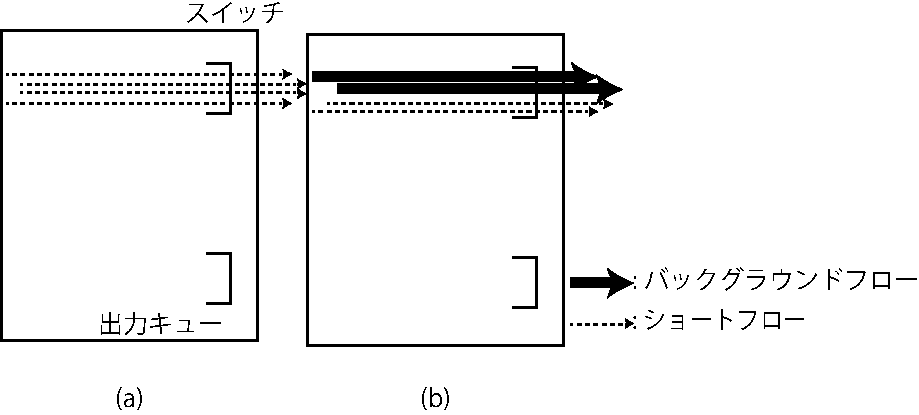
\includegraphics[autoebb, width=210pt]{./img/impairments.pdf}
    \caption{Two ways in which flows interact on a multi-ported switch
    resulting in performance problems.}
    \label{fig:impair}
    \end{center}
\end{figure}

% \section{再現シミュレーション実験}
% \label{sec:reproduction}
% この章では,
% Raiciuらによって示したFatTree-MPTCPネットワークモデルでのフローサイズの小さいトラフィックに対する性能評価シミュレーションを再現し,
% 解析を行った結果を示す.
%
% \subsection{再現シミュレーション実験環境}
% Raiciuらは~\cite{improving}において, 各プロトコルがフローサイズの小さなトラフィックに対して及ぼす影響の評価を行い,
% フローサイズの小さいトラフィックに関しては, MPTCPによりフロー完結時間を遅延させることを示した.
% そのときのシミュレーション環境は, 以下の通りである.
% ネットワークトポロジーには, 4:1にオーバーサブスクリプションされたFatTreeを用いている.
% ベンチマークトラフィックについては, ホスト同士の1対1通信を用いている.
% 全てのホストのうち, 33\%をTCPまたはMPTCPにより継続してデータ転送 (Background traffic)を行う.
% 残りのhostを使って, TCPによる70Kbyteのデータ転送(Short flow)を毎200[ms]のポアソン生起させ,
% 転送完了までにがかかった時間FCT(Flow Completion Time)を計測している.
%
% 今回の再現実験にはns-3 Direct Code Execution~\cite{ns3}を用い, MPTCPは, Linux
% カーネルソースを用いた~\cite{mptcp_linux}.
% 図\ref{fig:fattree_rep}に, シミュレーションで用いたFatTree(k=2)トポロジーを示す.
% このトポロジーでの物理パスでは, 一つのサブフローが1本の物理パスを占有するように, 設計している.
% すなわち, 4つのサブフローを使う場合, ホストの4インターフェースに対しそれぞれ4つIPアドレスが割り当てられる.
% また, Host-Edge部分には, IPアドレスの数だけインターフェースを用意し, Aggregation-Edge部分も,
% それに従いインターフェースを追加する.
% さらにルーティングに関しては, Core1$\sim$Core4に分散するようにルーティングテーブルを設定した.
%
% 表\ref{table:testbed}に再現シミュレーション環境に対する各パラメータをまとめる.
% \begin{table}[h]
% \begin{center}
% \footnotesize
% \begin{tabular}{c|c}
% \hline
% Parameter & Value \\ \hline \hline
% Nodes & 16 \\
% MPTCP & v0.88 \\
% Link core-aggr & 400Mbps \\
% Link aggr-edge & 200Mbps \\
% Link edge-host & 100Mbps \\
% RTT & 0.5ms\\
% Receive buffer size & 100KB \\
% \hline
% \end{tabular}
% \caption{Testbed on network simulation}
% \label{table:testbed}
% \end{center}
% \end{table}
%
% \begin{figure}[h]
%     \begin{center}
%     \includegraphics[autoebb, width=210pt]{./img/fattree_rep.pdf}
%     \caption{Network topology on reproducing simulation}
%     \label{fig:fattree_rep}
%     \end{center}
% \end{figure}
%
% \subsubsection{設定パラメータに対する有効性の検証}
% 伝搬遅延についてはRTT(Round Trip Time)として, 0.5[ms]に設定した.
% これは, 一般的なデータセンター内のRTTが1[ms]以下であるためである~\cite{rtt}.
%
% バッファサイズについては, 以下の帯域幅遅延積(BDP)の式から, 400Mbps$\times$4を最大限利用できるだけの値を設定した.
% \vspace{-2mm}
% \begin{eqnarray}
% BDP[{\rm byte}] = 帯域幅[{\rm bps}] \times RTT \div 8
% \label{cong}
% \vspace{-2mm}
% \end{eqnarray}
%
% 各帯域については, 16のノードを使って輻輳を引き起こす現象を再現するために, 実際のデータセンターのような広帯域のネットワークと比べ,
% 狭い帯域を設定した.
%
% \subsection{再現結果}
% 図\ref{fig:short_flow_rep}, 表\ref{table:short_flow_rep}に, 上記の実験環境で再現した結果を示す.
% 再現結果から, フローの様子を完結時間別に4パターンに分類することができることが分かった.
% 表\ref{table:flow_pattern}にそのフローパターンの定義を示す.
%
%
% 今回の再現実験において, TCPとMPTCPでフロー完結時間に差を生じた要因は, パケットロスが発生する割合にある.
% 図\ref{fig:cdf}に再現実験でのフロー完結時間ごとの累積確率分布を示す.
% パケットロスを生じないフローに関しては, 両者に性能差を感じなかったが, この図から, MPTCPを用いた方が,
% パケットロスを引き起こし遅延を生じさせる割合が大きいということが分かる.
%
% このようにMPTCPが帯域を大きく占有することにより他のトラフィックを圧迫することは, MPTCPの輻輳制御によるものだと考えられる.
% 混雑のない経路でデータ転送する場合, MPTCPでは積極的にウィンドウサイズを増やそうとするため, 他のフローに対し遅延を引き起こしたと推測される.
%
% \begin{figure}[h]
%     \begin{center}
%     \includegraphics[autoebb, width=210pt]{./img/flow_comp.pdf}
%     \caption{The result of the reproduction experiment}
%     \label{fig:short_flow_rep}
%     \end{center}
% \end{figure}
%
% \begin{figure}[h]
%     \begin{center}
%     \includegraphics[autoebb, width=210pt]{./img/cdf_rep.pdf}
%     \caption{CDF of flow completion time on reproduction experiment}
%     \label{fig:cdf}
%     \end{center}
% \end{figure}
%
% \begin{table}[h]
% \begin{center}
% \footnotesize
% \begin{tabular}{c|p{5em}|p{4em}|p{5em}}
% \hline
% Protocol & AVG comp time[ms]& Stdev[ms] &
% $95^{th}$ percentile[ms]\\
% \hline \hline TCP &\hfil 78.4 &\hfil 122.5 &\hfil 266.7\\
% MPTCP &\hfil 91 &\hfil 140.6 &\hfil 510.5\\
% \hline
% \end{tabular}
% \caption{Average flow completion time and stdev on reproduction experiment}
% \label{table:short_flow_rep}
% \end{center}
% \end{table}
%
% \begin{table}[h]
% \begin{center}
% \footnotesize
% \begin{tabular}{c|c|c}
% \hline
% Flow pattern & Comp time[ms] & Packet loss \\ \hline \hline
% Full window & $\sim$30 & \\
% Intensive flow & $\sim$60 & \\
% Delay with loss & 200$\sim$300 & $\surd$\\
% Extreme delay & 300$\sim$ & $\surd$\\
% \hline
% \end{tabular}
% \caption{Flow pattern classified by completion time}
% \label{table:flow_pattern}
% \end{center}
% \end{table}
%
%
%
% より詳細なMPTCPの影響を解析するため, 今回用いたFatTreeトポロジーを部分的に抽出したトポロジーを用いたシミュレーション環境により,
% どういった環境下でMPTCPによる影響を受け遅延が生じるのかを検証した.

\section{検証実験}
\label{sec:verification}
これまでの研究において報告されたMPTCPによるショートフロー性能劣化の問題~\cite{improving}を受け, その再現実験を行うことにより,
原因を解析し, 二つの要因を明らかにした~\cite{mptcp_ana}.
一つ目は, MPTCPはTCPよりも多くのトラフィックを排出する事で, パケットロスを伴う遅延が生じるということ.
二つ目は, MPTCPの実装上の問題から, 最大二つの経路しかデータ転送に利用できないということである.
これらの結果を受けて, MPTCPによるバックグラウンドトラフィックが利用している経路を回避し, 比較的輻輳が起こっていない経路を適切に選ぶ事で,
ショートフローのフロー完結時間(FCT)が改善できるのではないかと, 仮説を立てた.
この章では, シミュレーション実験を用いて, その仮説の検証, またMPTCPによるショートフローの遅延がどういった状況で発生するのかを明らかにする.

\subsection{再現シミュレーション実験環境}
ネットワークトポロジーには,
図\ref{fig:fattree_ver}のようなFatTreeを部分的に抽出した2:1にオーバーサブスクリプションされたトポロジーを用いる.
このトポロジーでの物理パスでは, 一つのサブフローが1本の物理パスを占有するように, 設計している.
すなわち, 4つのサブフローを使う場合, ホストの4インターフェースに対しそれぞれ4つIPアドレスが割り当てられる.
また, Host-Edge部分には, IPアドレスの数だけインターフェースを用意し, Aggregation-Edge部分も,
それに従いインターフェースを追加する.
さらにルーティングに関しては, Core1$\sim$Core4に分散するようにルーティングテーブルを設定した.
ベンチマークトラフィックについては, 二つのペアに対してホスト同士の1対1通信を用いている.
一方のペアに対しては, MPTCPにより継続してデータ転送 (バックグラウンドトラフィック)を行う.
他方のペアに対しては, TCPによる2$\sim$70Kbyteのデータ転送(ショートフロー)を毎200[ms]のポアソン生起させ,
転送完了までにがかかった時間FCT(Flow Completion Time)を計測している.

今回の再現実験にはns-3 Direct Code Execution~\cite{ns3}を用い, MPTCPは, Linux
カーネルソースを用いた~\cite{mptcp_linux}.
図\ref{fig:fattree_rep}に, シミュレーションで用いたFatTree(k=2)トポロジーを示す.


表\ref{table:testbed_ver}に再現シミュレーション環境に対する各パラメータをまとめる.
\begin{table}[h]
\begin{center}
\footnotesize
\begin{tabular}{c|c}
\hline
Parameter & Value \\ \hline \hline
Nodes & 4 \\
MPTCP & v0.88 \\
Link aggr-edge & 200Mbps \\
Link edge-host & 100Mbps \\
RTT & 0.5ms\\
Receive buffer size & 50KB \\
\hline
\end{tabular}
\caption{Testbed on verificating simulation}
\label{table:testbed_ver}
\end{center}
\end{table}

\begin{figure}[h]
    \begin{center}
    \includegraphics[autoebb, width=210pt]{./img/fattree_part.pdf}
    \caption{Network topology on verificating simulation}
    \label{fig:fattree_ver}
    \end{center}
\end{figure}

\subsubsection{設定パラメータに対する有効性の検証}
伝搬遅延についてはRTT(Round Trip Time)として, 0.5[ms]に設定した.
これは, 一般的なデータセンター内のRTTが1[ms]以下であるためである~\cite{rtt}.

バッファサイズについては, 以下の帯域幅遅延積(BDP)の式から, 200Mbps$\times$4を最大限利用できるだけの値を設定した.
\vspace{-2mm}
\begin{eqnarray}
BDP[{\rm byte}] = 帯域幅[{\rm bps}] \times RTT \div 8
\label{cong}
\vspace{-2mm}
\end{eqnarray}

各帯域については, 4のノードを使って輻輳を引き起こす現象を再現するために, 実際のデータセンターのような広帯域のネットワークと比べ,
狭い帯域を設定した.

\subsection{検証結果}
図\ref{fig:improve}に上記の実験環境での結果として, 70KBのショートフローのFCTとそれぞれの経路の利用率を示す.
この結果から, background trafficよるリンク利用率の高いpath1, path2において, FCTの分散が大きくなっている事が分かる.
これは, 大部分のフローは遅延が生じる事なく完結できるが, 遅延が生じる割合, またその遅延量が大きくなることを示している.
実際に, 図\ref{fig:95percentile}においてはフローサイズを変え, FCTの大きかった下位5\%に着目したグラフであるが,
利用率の大きいpath1, path2と比較し, path3, path4におけるショートフローのFCTは, 最もサイズの小さい2[kb]フローにおいても10[ms]程度の差があった.

また, 図\ref{fig:inter-flow}では平均200[ms]でポアソン生起するフローの発生間隔と遅延が生じるフローの関係を示している.
この結果から, フローの発生間隔が短く, 複数のフローが同時刻に混在する状況において, 遅延が生じる事が分かる.
% このことは図\ref{}のフローの生起間隔を一定値として変化させた時の70[kb]FCTでも明らかである.

これらの事から, 遅延を引き起こす要素としては, 「リンク利用率」, 「フロー発生間隔」があると考えられ, それぞれ, Queue buildup,
Incastを引き起こす要因となる.

\begin{figure}[h]
    \begin{center}
    \includegraphics[autoebb, width=210pt]{./img/70kb_fix.pdf}
    \caption{Flow completion time and link utilization for 70kb benchmark
    traffic}
    \label{fig:improve}
    \end{center}
\end{figure}

\begin{figure}[h]
    \begin{center}
    \includegraphics[autoebb, width=210pt]{./img/95percentile.pdf}
    \caption{95 percentile FCT for 70kb flow}
    \label{fig:95percentile}
    \end{center}
\end{figure}

\begin{figure}[h]
    \begin{center}
    \includegraphics[autoebb, width=210pt]{./img/inter_flow.pdf}
    \caption{Inter-flow with percentile for 70kb benchmark
    traffic}
    \label{fig:inter-flow}
    \end{center}
\end{figure}

\subsubsection{リンク利用率の影響}
リンク利用率による遅延の影響がどのように生じているのかを解析するため, 各スイッチでキャプチャしたpcapデータを基にして,
バックグラウンドトラフィックの有無によるパケット発生間隔の変化の解析を行った.
pcapデータにはpath1における70kbフローを用いた.
すなわち, バックグラウンドトラフィック有の場合には, 一つの経路に二つのフローが混在する事になる.
図\ref{fig:inter-packet}にパケット発生間隔の差分の累積を示す.
この差分の値が大きければ大きいほど, そのホストにおけるキューイング遅延が大きかった事を示している.
バックグラウンドトラフィックが流れている時のSenderホスト-Edgeスイッチ間でのパケット発生間隔の変化から,
Edgeスイッチのキューイング遅延がボトルネックとなっている事が分かり, Queue buildupでの性能障害が起きていることが分かる.

\begin{figure}[h]
    \begin{center}
    \includegraphics[autoebb, width=210pt]{./img/inter_packet.pdf}
    \caption{Inter-flow with/without bankground traffic for 70kb benchmark
    traffic}
    \label{fig:inter-packet}
    \end{center}
\end{figure}

\subsubsection{フロー発生間隔の影響}
短いフロー発生間隔におけるフロー多重化による遅延の影響がどのように生じているのかを解析するため, 各スイッチでキャプチャしたpcapデータを基にして,
よるパケット発生間隔の変化の解析を行った.
pcapデータには70kbフローのみを用い, フロー発生間隔は50, 200[ms]でそれぞれのFCTを比較した.
図\ref{fig:detail}にフローが完結するまでの通信の様子を示す.
発生間隔200[ms]のフローでは, 滞りなくデータ転送を130ms程度で完了し, 後続のフローとは競合しないことが分かる.
発生間隔50[ms]のフローでは, 段階的にデータを送り, 待ちが発生している様子が分かるが, これは, 待ちの間に他のフローの通信を行っているからであり,
インターフェース単位で見ると常に一定したデータを送信している.
そのため, 各フロー毎の完結時間の遅延が生じる.

\begin{figure}[h]
    \begin{center}
    \includegraphics[autoebb, width=210pt]{./img/detail.pdf}
    \caption{Detail receiving 70kb flow}
    \label{fig:detail}
    \end{center}
\end{figure}


\subsection{考察}
\label{sec:analysis}
これらの解析結果から, \ref{sec:switch}小節にて示した二つの機能障害が引き起こる要因について述べ, 今後の改善手法の検討を行う.\\
{\bf Queue buildup: }フローサイズが大きく,
長時間データを通信し続けるバックグラウンドトラフィックの影響によって中継するスイッチのキューサイズは大きく保たれてしまい,
そのポートにおけるキューイング遅延が生じる.
その中でフローサイズが小さく, 本質的には短時間で完結できるフローが, 同じポートを使って通信する事で,
キューイング遅延やキュー溢れによるパケットロスの影響を受け, フロー完結時間が大きくなる.
そうした遅延の影響が引き起こる為には, 同時に多数のショートフローは必要でなく, バックグラウンドトラフィックがキューを圧迫している状況で,
他のフローが流入する事により生じる.\\
{\bf Incast: }サイズの小さいフローが多数生成され, それらのフローが短期間にアグリゲートホストに流入しようし,
アグリゲートホストが接続されているスイッチのポートにトラフィックが集中する事で, バッファが圧迫される事によりキューイング遅延, パケットロスが生じる結果,
それぞれのフローの完結時間が大きくなる.
そうした遅延の影響が引き起こる為には, 各ホストにおけるショートフローの発生間隔が小さい時に, 複数のフローが同時刻に通信を行うことにより生じる.

こうした遅延の影響を軽減する為には, 通信を行うスイッチポートのキューサイズを小さく保ち, 通信を行う事が重要である.
具体的には, 図\ref{fig:improve}に示すように, 同じスイッチでも異なる物理ポートを用いる,
あるいはRaiciuらが提案しているDual-Homed FatTreeのようなEdgeスイッチを複数設けたトポロジーを用いる事で,
物理的に異なるスイッチを中継する事でキューが圧迫の問題を回避できると考える~\cite{improving}.
こうした経路の切り替えを既存の仕組みを用いて実現する事を考えると, MPTCPの持つ輻輳制御アルゴリズムに対して新たなアルゴリズムを提案する必要があると考える.
実際, MPTCP輻輳制御に関しては議論が行われており, TCPとの親和性と経路状況への対応とのトレードオフの関係性から様々なアルゴリズム提案されている.
上記のような遅延の問題を解決する為に, MPTCPの輻輳制御を用いて経路を切り替える事を実現するならば,
従来の制御よりも経路の状況により機敏に対応できる経路切り替えに特化した輻輳制御アルゴリズムが必要であると考えられる.

% \subsubsection{Background traffic}
% Background
% trafficに対する評価として全12の処理ノードへ平均500[ms]のポアソン生起でフローサイズ1[KB]$\sim$1[MB]のトラフィックを同時に発生させた状態で,
% 同時に12の処理ノードへ平均500[ms]のポアソン生起でトラフィックを発生させ, 各経路のスループットを計測した.
% その結果を図\ref{fig:background}に示す.
%
% この結果から, MPTCPはBackground trafficに対し, TCPよりも性能向上が見られることが分かる.
% これは, MPTCPのロードバランスと複数経路を使って並行的にデータを送信したことによるものである.
%
% \begin{figure}[h]
%     \begin{center}
%     \includegraphics[autoebb, width=180pt]{./img/back.pdf}
%     \caption{Throughput of background traffic}
%     \label{fig:background}
%     \end{center}
% \end{figure}
% \hspace{1cm}

\section{あとがき}
\label{sec:conclude}
本論文では, サイズが大きく長時間通信を行うバックグラウンドトラフィックとサイズが小さくフロー完結時間を短く抑えたいショートフローが混在する状況において, フローサイズの小さいトラフィックに対しては,
従来のTCPよりもデータ転送に時間がかかるという報告~\cite{improving}を再現し, その原因を分析した.
その結果, ショートフローが通信で用いるリンクの利用率とフローが発生する間隔の二つの要因がショートフローの遅延に影響を及ぼす事を示した.
特に, アグリゲートスイッチにおけるキューイングのボトルネックになっており, その問題に対して通信経路を切り替える事によりフロー完結時間を改善した事を示した.
このことから, キューサイズが大きくなっているスイッチポートを回避するような経路において通信を行う事をMPTCPの輻輳制御によって実現する事で,
フローサイズの小さいトラフィックの完結時間を短縮化し, 並列分散処理のパフォーマンスの改善が期待される.

今後は実機を用いてキューイングの問題を再現し, それを回避するネットワークトポロジーとMPTCPの輻輳制御の提案を行う.
%\bibliographystyle{sieicej}
%\bibliography{myrefs}
\begin{spacing}{0.7}
\footnotesize{
\begin{thebibliography}{99}% 文献数が10未満の時 {9}
\bibitem{IBM_rep}{日本アイ・ビー・エム株式会社. IBM 第1章
大容量データのバックアップ,
\url{http://www-06.ibm.com/systems/jp/storage/column/backup/01.html}} \bibitem{amazon}{Jim Liddle. Amazon found every 100ms of latency cost them 1\%
in sales, August 2008.
\url{http://blog.gigaspaces.com/amazon-found-every-100ms-of-latency-cost}

\url{-them-1-in-sales/}}
\bibitem{presto}{Facebook. Presto: Interacting with petabytes
of data at Facebook,
\url{https://www.facebook.com/notes/facebook-engineering/presto-interacting-with-petabytes-of-data}

\url{-at-facebook/10151786197628920}}
\bibitem{mapreduce}{Dean, Jeffrey, and Sanjay
Ghemawat. "MapReduce: simplified data processing on large clusters." Communications of the ACM 51.1 (2008): 107-113.} \bibitem{dryad}{Isard, Michael, et al. "Dryad: distributed data-parallel
programs from sequential building blocks." ACM SIGOPS Operating Systems Review 41.3 (2007): 59-72.}
\bibitem{fattree}{Al-Fares, Mohammad, Alexander Loukissas, and Amin Vahdat. "A
scalable, commodity data center network architecture." ACM SIGCOMM Computer Communication Review. Vol. 38. No. 4. ACM, 2008.}
\bibitem{bcube}{Guo, Chuanxiong, et al. "BCube: a high performance,
server-centric network architecture for modular data centers." ACM SIGCOMM Computer Communication Review 39.4 (2009): 63-74.}
\bibitem{vl2}{Greenberg, Albert, et al. "VL2: a scalable and flexible data
center network." ACM SIGCOMM Computer Communication Review. Vol. 39. No. 4. ACM, 2009.}
\bibitem{dctcp}{Alizadeh, Mohammad, et al. "Data center tcp (dctcp)." ACM SIGCOMM Computer Communication Review 40.4 (2010): 63-74.}
\bibitem{improving}{Raiciu, Costin, et al. "Improving datacenter performance and
robustness with multipath TCP." ACM SIGCOMM Computer Communication Review. Vol. 41. No. 4. ACM, 2011.}
\bibitem{detail}{Zats, David, et al. "DeTail: Reducing the flow completion time
tail in datacenter networks." ACM SIGCOMM Computer Communication Review 42.4 (2012): 139-150.}
\bibitem{p_fab}{Alizadeh, Mohammad, et al. "pfabric: Minimal near-optimal datacenter transport." Proceedings of the ACM SIGCOMM 2013 conference on SIGCOMM. ACM, 2013.}
\bibitem{click}{Kohler, Eddie, et al. "The Click modular router." ACM
Transactions on Computer Systems (TOCS) 18.3 (2000): 263-297.}
\bibitem{mptcp}{Ford, Alan, et al. TCP Extensions for Multipath Operation with
Multiple Addresses: draft-ietf-mptcp-multiaddressed-03. No. Internet draft (draft-ietf-mptcp-multiaddressed-07). Roke Manor, 2011.}
\bibitem{cong}{Raiciu, C., M. Handley, and D. Wischik. "Coupled congestion
control for multipath transport protocols." draft-ietf-mptcp-congestion-01 (work in progress) (2011).}
\bibitem{ns3}{Inria「DCE - GETTING STARTED Direct Code Execution」
\url{http://www.nsnam.org/~thehajime/ns-3-dce-doc/getting-started.html}}
\bibitem{traffic}{Benson, Theophilus, Aditya Akella, and David A. Maltz.
"Network traffic characteristics of data centers in the wild." Proceedings of the 10th ACM SIGCOMM conference on Internet measurement. ACM, 2010.}
\bibitem{mptcp_linux}{ip networking lab「MultiPath TCP - Linux Kernel
implementation」\url{http://mptcp.info.ucl.ac.be/}}
\bibitem{rtt}{Vasudevan, Vijay, et al. "Safe and effective fine-grained TCP
retransmissions for datacenter communication." ACM SIGCOMM Computer Communication Review. Vol. 39. No. 4. ACM, 2009.}
\bibitem{mptcp_ana}{藤居 翔吾, 田崎 創, 関谷 勇司, "MultiPath TCP
適用時のデータセンターネットワークでのフローサイズが与える影響に関する一考察", 電子情報通信学会, 信学技法, vol. 113, no. 364,
IA2013-65, pp. 47-52, 2013.P. Agarwal, B. Kwan, and L. Ashvin. Flexible buffer allocation entities for
traffic aggregate containment. US Patent 20090207848, August 2009.}
\bibitem{flexible}{P. Agarwal, B. Kwan, and L. Ashvin. Flexible buffer allocation entities for
traffic aggregate containment. US Patent 20090207848, August 2009.}
\bibitem{synchro}{S. Floyd and V. Jacobson. The synchronization of periodic routing messages.
IEEE/ACM ToN, 1994.}
\bibitem{balia}{A. Walid, et al. Balanced Linked Adaptation Congestion Control
Algorithm for MPTCP draft-walid-mptcp-congestion-control-00, 2014.}

\end{thebibliography}
}
\end{spacing}


\end{document}